\documentclass[xcolor={dvipsnames}]{beamer}
\usepackage{color, colortbl}
\usepackage[ngerman,english]{babel}
\usepackage[T1]{fontenc}
\usepackage{CJKutf8} %japanese
\usepackage{lmodern}
\usepackage[compatibility=false]{caption}
\usepackage{subcaption}
\usepackage{tikz}
\usepackage{textgreek}
\usepackage{tabularx}
\usepackage{booktabs}
\usepackage{siunitx}
\usepackage{appendixnumberbeamer}
\usepackage[absolute,overlay]{textpos} %for positioning the logos where I want
\usepackage{xspace,multicol}

\usepackage{animate}
\usepackage{multimedia}

\usepackage{amsfonts} % for the \checkmark command 

\mode<presentation>
{
  \usetheme{CambridgeUS}     
  \usecolortheme{lily} 
  \definecolor{beamer@violet}{rgb}{0.5,0.3,0.5} % changed this
  \setbeamercolor{structure}{fg=beamer@violet!70!cyan}
  \setbeamercolor{palette primary}{fg=black, bg=gray!30!white!50!cyan!20!}
  \setbeamercolor{palette secondary}{fg=black, bg=gray!30!white!30!cyan!40!}
  \setbeamercolor*{palette tertiary}{bg=gray!20!white!20!cyan!60!}
  
  \setbeamercolor{frametitle}{fg=cyan!60!white!40!,bg=cyan!80!black}
  \setbeamercolor{title}{fg=cyan!80!black}
  \setbeamercolor{normal text}{fg=black,bg=white}
  \setbeamercolor{alerted text}{fg=beamer@violet}
  \setbeamercolor{example text}{fg=beamer@violet!70!cyan}
  
  \usefonttheme{structureitalicserif} 
  \setbeamertemplate{navigation symbols}{}
  \setbeamertemplate{caption}[numbered]
}
\newcommand{\sidlogo}{
  \setlength{\TPHorizModule}{1pt}
  \setlength{\TPVertModule}{1pt}
   % textblock{}{x,y}: pos(x) = rightUpperCorner + (x * \TPHorizModule), pos(y) = leftUpperCorner - (y * \TPVertModule)
  \begin{textblock}{1}(323,12)
   \includegraphics[width=40pt,height=26pt]{figures/SiD.jpeg}
  \end{textblock}
  } 
\newcommand{\ilclogo}{
  \setlength{\TPHorizModule}{1pt}
  \setlength{\TPVertModule}{1pt}
   % textblock{}{x,y}: pos(x) = rightUpperCorner + (x * \TPHorizModule), pos(y) = leftUpperCorner - (y * \TPVertModule)
  \begin{textblock}{1}(323,12)
   \includegraphics[width=40pt,height=26pt]{figures/ILC.jpeg}
  \end{textblock}
} 
\newcommand{\flukalogo}{
  \setlength{\TPHorizModule}{1pt}
  \setlength{\TPVertModule}{1pt}
   % textblock{}{x,y}: pos(x) = rightUpperCorner + (x * \TPHorizModule), pos(y) = leftUpperCorner - (y * \TPVertModule)
  \begin{textblock}{1}(315,12)
   \includegraphics[width=60pt,height=26pt]{figures/fluka_logo.png}
  \end{textblock}
} 
\newcommand{\ejadelogo}{
  \setlength{\TPHorizModule}{1pt}
  \setlength{\TPVertModule}{1pt}
   % textblock{}{x,y}: pos(x) = rightUpperCorner + (x * \TPHorizModule), pos(y) = leftUpperCorner - (y * \TPVertModule)
  \begin{textblock}{1}(323,12)
   \includegraphics[width=40pt,height=26pt]{figures/EJADE.jpeg}
  \end{textblock}
} 
\newcommand{\BDSsymbol}{
  \setlength{\TPHorizModule}{1pt}
  \setlength{\TPVertModule}{1pt}
   % textblock{}{x,y}: pos(x) = rightUpperCorner + (x * \TPHorizModule), pos(y) = leftUpperCorner - (y * \TPVertModule)
  \begin{textblock}{1}(0,39)
   \includegraphics[width=60pt,height=40pt]{figures/Highlight_BDS.png}
  \end{textblock}
} 
\newcommand{\EXTsymbol}{
  \setlength{\TPHorizModule}{1pt}
  \setlength{\TPVertModule}{1pt}
   % textblock{}{x,y}: pos(x) = rightUpperCorner + (x * \TPHorizModule), pos(y) = leftUpperCorner - (y * \TPVertModule)
  \begin{textblock}{1}(0,39)
   \includegraphics[width=60pt,height=40pt]{figures/Highlight_EXT.png}
  \end{textblock}
} 
\newcommand{\ATFlogo}{
  \setlength{\TPHorizModule}{1pt}
  \setlength{\TPVertModule}{1pt}
   % textblock{}{x,y}: pos(x) = rightUpperCorner + (x * \TPHorizModule), pos(y) = leftUpperCorner - (y * \TPVertModule)
  \begin{textblock}{1}(323,12)
   \includegraphics[width=40pt,height=26pt]{figures/ATF_logo.jpg}
  \end{textblock}
} 
\newcommand{\RHULlogo}{
  \setlength{\TPHorizModule}{1pt}
  \setlength{\TPVertModule}{1pt}
   % textblock{}{x,y}: pos(x) = rightUpperCorner + (x * \TPHorizModule), pos(y) = leftUpperCorner - (y * \TPVertModule)
  \begin{textblock}{1}(337,12)
   \includegraphics[width=25pt,height=26pt]{figures/rhul_logo.png}
  \end{textblock}
}

\DeclareSIUnit\year{yr}
\newcommand{\eplus}{e$^+$\xspace}
\newcommand{\eminus}{e$^-$\xspace}


\title[ATF2 Background Simulations]{\textbf{BDSIM simulation model of ATF2 \& Background Studies\\for the Vertical Collimator System}}
\author{\textbf{Anne Sch\"utz}}
\institute{\textbf{KIT, DESY}}
\date{\textbf{April 10, 2017}}

\titlegraphic{
  %\includegraphics[height=1.1cm]{figures/EJADE.png}\hspace*{0.5cm}~%
  \includegraphics[height=1.0cm]{figures/KIT.png}\hspace*{2cm}~%
    \includegraphics[height=1.0cm]{figures/ATF_logo.jpg}\hspace*{3cm}~%
  \includegraphics[height=1.1cm]{figures/DESY_Logo.png}
  %\includegraphics[height=1.0cm]{figures/rhul_logo.png}\hspace*{0.5cm}~%
  %\includegraphics[height=1.0cm]{figures/ific_logo.png}
}

\begin{document}

{
\usebackgroundtemplate{
 \tikz\node[opacity=0.1]{\includegraphics[width=\paperwidth]{figures/Iwatecomics.jpg}};
 % \tikz\node[opacity=0.2]{\centering\includegraphics[height=\paperheight]{figures/Iwatecomics.jpg}};
 }
\begin{frame}
  \titlepage
\end{frame}
}

\begin{frame}{Table of contents}
  \tableofcontents
\end{frame}

%--------------------------------------------------------------

\section{BDSIM simulations}
\begin{frame}
Original strategy for BDSIM simulations, and things that have been done already thanks to the RHUL BDSIM group:
\begin{itemize}
    \item[\checkmark] Using PyGDML for modelling the vertical collimator
    \item[\checkmark] Setting up BDSIM on the DESY NFS system, so that BDSIM jobs can be sent to the DESY BIRD cluster
    \item[\checkmark] Writing analysis code (e.g. AnalysisUser) to compare taken data to simulation, and to find origins of secondary particles, i.e. background
    \item[\checkmark] Putting together all new component models for a more accurate ATF geometry model
    \item[$\times$] More accurate Aperture Model of ATF2 (especially at places with large beta)
    \item[$\times$] Studying effect of the tapered beam pipe (collimator) on background level at the RHUL cherenkov detector and the IP
    \item[$\times$] Introducing beam bumps in simulation to study the effect of beam orbit changes  on background level at the RHUL cherenkov detector and the IP
    \item[$\times$] Changing vacuum pressure in the simulation to also compare these data taken
\end{itemize}

\end{frame}

\AtBeginSubsection[]
{
  \begin{frame}<beamer>
     \tableofcontents[currentsection,
     currentsubsection,
     %hideothersubsections,
     subsectionstyle=show/shaded/hide]
  \end{frame}
}

\subsection{Using PyGDML for the Collimator Model}
\begin{frame}{Modelling the Vertical Beam Halo Collimator}
\ATFlogo
\begin{center}
View inside the collimator model \hspace*{1cm} Collimator in ATF2 beam line\\
\vspace*{0.2cm}
 \includegraphics[width=0.5\textwidth]{figures/Collimator_model.pdf}
 \includegraphics[width=0.5\textwidth]{figures/Collimator_in_ATF2.png}
\end{center}
The collimator was modelled with \textbf{PyGDML} according to the technical drawings provided by Nuria Fuster Martinez.\\
Its jaws can be placed as desired.
$\Rightarrow$ Individual jaw movement is now possible!\\
\vspace*{0.2cm}
Jaws are not modelled correctly, because ``Trap'' class within PyGDML is not completed yet.
\end{frame}

\subsection{Running BDSIM on the BIRD cluster at DESY}
\begin{frame}
\RHULlogo
Stewart has set up BDSIM at DESY:
\begin{itemize}
 \item locally in my NFS folder
 \item here: (accessable if permissions given)\\
 /afs/desy.de/user/i/iagapov/xxl/mpy/colsim/bdsim-rhul/accsoft/
\end{itemize}
\vspace*{0.2cm}
Use BDSIM by doing:\\
\textcolor{Gray}{\texttt{\small source /etc/profile.d/modules.sh\\                                                
module use {\footnotesize /afs/desy.de/user/i/iagapov/xxl/mpy/colsim/bdsim-rhul/accsoft/modules/all}\\
module load Bdsim\\
source \$EBROOTGEANT4/bin/geant4.sh\\
bdsim --file=atf2.gmad
}}\\
\vspace*{0.2cm}
Submitting jobs to the BIRD cluster for all vertical collimator settings:\\
50 settings, $\sim$ 100 jobs each, 10000 initial particles per job\\
$\rightarrow$ \textit{10000 particles only because BDSIM would enter ``infinite'' loop for very low momentum particles}
\end{frame}

\subsection{ATF2 optics \& ATF2 model}
\begin{frame}{$\sigma$ and $\beta$ as function of S}
Running BDSIM with the beam core, large beam pipe radius (240mm) and collimators as drifts. 
Then running rebdsim on the output files.\\
With the gmad file from Nuria:
 \includegraphics[width=0.5\textwidth]{figures/histo_beta_s.pdf}
 \includegraphics[width=0.5\textwidth]{figures/histo_sigma_s.pdf}\\
Large beam sizes, but fine at IP (S = 38m).\\
\textcolor{Gray}{Vertical collimator: S = 9.25m\\
RHUL Cherenkov detector: S = 17.75m}
\end{frame}

\begin{frame}{Test optics}
With PyBDSIM, compare MADX tfs file of ATF with the rebdsim analysis output.\\
 \includegraphics[width=0.9\textwidth]{figures/pybdsim_sigma_gmadNuria.png}\\
Optics seem to be fine!
\end{frame}

\begin{frame}{Putting together new component models}
List of all ATF magnets and their types:\\
\vspace*{0.5cm}
\includegraphics[width=0.9\textwidth]{figures/RHUL_Twiki_ATFmagnets.png}
\end{frame}

\begin{frame}{Putting together new component models}
Python script that adds the gdml file paths to the atf\_components.gmad file when generated from MADX tfs file:\\
\vspace*{0.2cm}
\textcolor{Gray}{\texttt{\small pybdsim.Convert.MadxTfs2Gmad(\\
"./twiss\_v5.2.tfs","atf2",flipmagnets=True,\\
\textbf{collimatordict}=\{\\
'COLLBY' : \{'outerDiameter':0.8, 'geometryFile' : 'gdml:/scratch/atf2model/geom/collimator/realistic\_collim.gdml'\}\},\\
\textbf{userdict}=\{\\
\# Damping ring:\\
\#'KEX1A' : \{'geometry' : 'gdml:/scratch/atf2model/geom/mag/'\},\\
\#'KEX1B' : \{'geometry' : 'gdml:/scratch/atf2model/geom/mag/'\},\\
'QM6RX' : \{'geometry' : 'gdml:/scratch/atf2model/geom/mag/hitachi/hitachiIV.gdml'\},\\
...)
}}\\
\vspace*{0.2cm}
I commented out the ones without available gdml file.
\end{frame}


\begin{frame}{Putting together new component models}
The atf\_components.gmad file then looks like:\\
\textcolor{Gray}{\texttt{\small ! Mon, 10 Apr 2017 08:43:40 +0000\\
! pybdsim.Builder Lattice \\
! COMPONENT DEFINITION\\
KEX1A: sbend, angle=0.0025, fint=0.5, l=0.2500010417;\\
KEX1B: sbend, angle=0.0025, l=0.2500010417, fintx=0.5, e2=0.005;\\
L001: drift, l=0.9231390392;\\
QM6RX: sbend, geometry="gdml:/scratch/atf2model/geom/mag/hitachi/hitachiIV.gdml", k1=3.66724845038, angle=0.0023109657, l=0.09937458845;\\
...
}}\\
If gdml addition in userdict, the length is still be taken from the tfs file, not the gdml file.
$\rightarrow$ Different values! Which one is correct?\\
\vspace*{0.2cm}
In ``withgeometry'' branch of the ``atf2model'' repository, atf2\_magnetgeom.gmad:\\
\textcolor{Gray}{\texttt{\small 
QF1X: magnetGeometryType="gdml:geom/hitachiVhalf.gdml";\\
QF1X\_1: magnetGeometryType="gdml:geom/hitachiVhalf.gdml";
}}
\end{frame}

\begin{frame}{Test optics - Final Focus}
Again, with PyBDSIM, compare MADX tfs file of ATF with the rebdsim analysis output.\\
 \includegraphics[width=0.5\textwidth]{figures/sigma_COLLdrifts.png}
 \includegraphics[width=0.5\textwidth]{figures/sigma2_COLLdrifts.png}\\
Good agreement in beginning, then phase shift?
\end{frame}

\begin{frame}{Test optics - Whole ATF}
Again, with PyBDSIM, compare MADX tfs file of ATF with the rebdsim analysis output.\\
 \includegraphics[width=0.5\textwidth]{figures/wholeATF_sigma_COLLdrifts.png}
 \includegraphics[width=0.5\textwidth]{figures/wholeATF_sigma2_COLLdrifts.png}\\
Some agreement 
\end{frame}


\section{Background studies for the Vertical Collimator System}

\subsection{Background Measurements at ATF2}
\begin{frame}{The Vertical Beam Halo Collimator and the\\RHUL Cherenkov detector}
\ATFlogo
\begin{center}
\includegraphics[width=\textwidth]{figures/ATF2schematic.pdf}\\
  \includegraphics[width=\textwidth]{figures/RHUL_detector_Collimator.png}
\end{center}
\end{frame}

\begin{frame}{Background Data taken with the RHUL Cherenkov detector}
\ATFlogo
\begin{center}
 Symmentric jaw movement \hspace*{2.5cm} Jaws moving separately\\
\vspace*{0.2cm}
 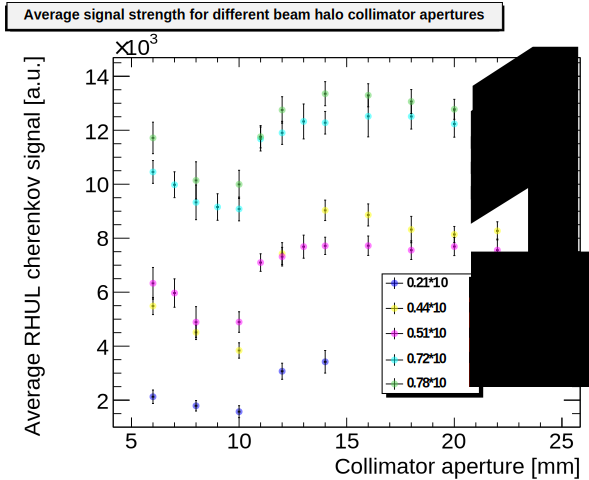
\includegraphics[width=0.55\textwidth]{figures/AverageSignal_perAperture.pdf}
  \includegraphics[width=0.55\textwidth]{figures/AverageSignal_perJawPosition_12April2016.pdf}
\end{center}
Background is reduced, but then rises again when collimator jaws are driven closer into the beam halo.\\
Individual jaw movement gives conflicting results.
%\begin{block}{}
%The vertical beam size at the location of the collimator was about \SI{0.32}{mm} with an offset of 0.2-\SI{0.5}{mm}.
%\end{block}
\end{frame}

\subsection{Analysis objectives}
\begin{frame}
Plots that I produce:
 \begin{itemize}
  \item data/MC comparison of the RHUL detector signal in dependency of the collimator aperture
  \item the number of particles created in the single ATF2 beam line components
  \item the number of particles created in the single ATF2 beam line components, hitting:
  \begin{itemize}
   \item the vertical collimator (COLLBY)
   \item the RHUL cherenkov detector (RHUL\_detector2)
   \item the IP (IP)
  \end{itemize}
 \end{itemize}

\end{frame}


\subsection{Data to MC comparison}
\begin{frame}{First Data to MC comparison}
\ATFlogo
\begin{center}
\includegraphics[width=0.7\textwidth]{figures/data_mc_comparison.pdf}
\end{center}
First data to MC comparison is not satisfactory.\\
The ATF2 model in BDSIM needs to be reviewed.
\end{frame}

\subsection{Vertex studies}
\begin{frame}{Study of the ATF2 components producing secondary particles}
 \begin{center}
 \only<1>{
\includegraphics[width=0.38\textwidth]{figures/TracksPerModel_firstPart.pdf}
\includegraphics[width=0.38\textwidth]{figures/TracksPerModel_secondPart.pdf}\\
\includegraphics[width=0.38\textwidth]{figures/TracksPerModel_thirdPart.pdf}
\includegraphics[width=0.38\textwidth]{figures/TracksPerModel_forthPart.pdf}\\
Number of particles created in the components of the ATF2 beam line.
}
 \only<2>{
 \begin{columns}
  \begin{column}{0.3\textwidth} 
   \includegraphics[angle=270,width=\textwidth]{figures/ATF2_beamline_firstPart.png}
  \end{column}
 \begin{column}{0.8\textwidth} 
\includegraphics[width=\textwidth]{figures/TracksPerModel_firstPart.pdf}
  \end{column}
 \end{columns}
}
 \only<3>{
  \begin{columns}
  \begin{column}{0.3\textwidth} 
   \includegraphics[angle=270,width=0.7\textwidth]{figures/ATF2_beamline_secondPart.png}
  \end{column}
 \begin{column}{0.8\textwidth}
\includegraphics[width=\textwidth]{figures/TracksPerModel_secondPart.pdf}
  \end{column}
 \end{columns}
}
 \only<4>{
  \begin{columns}
  \begin{column}{0.3\textwidth} 
   \includegraphics[angle=270,width=\textwidth]{figures/ATF2_beamline_thirdPart.png}
  \end{column}
 \begin{column}{0.8\textwidth}
\includegraphics[width=\textwidth]{figures/TracksPerModel_thirdPart.pdf}
  \end{column}
 \end{columns}
}
 \only<5>{
  \begin{columns}
  \begin{column}{0.3\textwidth} 
   \includegraphics[angle=270,width=\textwidth]{figures/ATF2_beamline_forthPart.png}
  \end{column}
 \begin{column}{0.75\textwidth}
\includegraphics[width=\textwidth]{figures/TracksPerModel_forthPart.pdf}
  \end{column}
 \end{columns}
}
\end{center}
\end{frame}

\begin{frame}{Study of the ATF2 components producing secondary particles, sampled in the Vertical Collimator}
These components create particles hitting explicitly the Vertical Collimator:
 \begin{center}
\includegraphics[width=0.6\textwidth]{figures/VertexModels_Comparison_Sampler0.pdf}
\end{center}
\end{frame}
\begin{frame}{Study of the ATF2 components producing secondary particles, sampled in the RHUL detector}
These components create particles hitting the RHUL detector plane:
 \begin{center}
\includegraphics[width=0.6\textwidth]{figures/VertexModels_Comparison_Sampler1.pdf}
\end{center}
\end{frame}
\begin{frame}{Study of the ATF2 components producing secondary particles, sampled in the IP}
These components create particles that reach explicitly the IP:
 \begin{center}
\includegraphics[width=0.6\textwidth]{figures/VertexModels_Comparison_Sampler2.pdf}
\end{center}
\end{frame}

\section{Outlook}
\begin{frame}{BDSIM simulation: Outlook}
\ATFlogo
Possible plan for cross checking the ATF2 model \& hopefully correcting the data/MC comparison:\\
\begin{itemize}
 \item Improve the Vertical Collimator model
 \item Reviewing the BDSIM geometry model of ATF2 (large sigma at IP!)
 \item More accurate Aperture Model of ATF2 (especially at places with large beta)
\end{itemize}
When the first data to MC comparison looks fine, then:
\begin{itemize}
 \item Study the effect of the tapered beam pipe
 \item Introduce beam bumps in simulation to study effect of beam orbit changes on background level at the RHUL cherenkov detector and the IP
 \item Change vacuum pressure in the simulation to also compare these data taken
\end{itemize}

\end{frame}



\section*{The end}
{
\usebackgroundtemplate{
 \tikz\node[opacity=0.1]{\includegraphics[width=\paperwidth,resolution=200]{figures/ilc-Comic.png}};
 % \tikz\node[opacity=0.2]{\centering\includegraphics[height=\paperheight]{figures/Iwatecomics.jpg}};
 }
\begin{frame}
\ATFlogo
\begin{center}
\textcolor{RubineRed}{
	\LARGE Thank you very much!\\
	%\vspace*{0.5cm}
	%\begin{CJK}{UTF8}{min}
	%どうもありがとうございます。
	%\end{CJK}
}
\end{center}
\end{frame}
}

%--------------------------------------------------------------------------------
\appendix

\begin{frame}
\begin{center}
\LARGE Additional Material
\end{center}
\end{frame}

\AtBeginSection[]
{
  \begin{frame}<beamer>
     \tableofcontents[currentsection,
     hideothersubsections]
  \end{frame}
}

\section{The Tapered Beam Pipe}
\begin{frame}
 \includegraphics[width=\textwidth]{figures/TBP2.png}\\
 In atf2\_components.gmad:\\
 {\small COLL: ecol, l=0.094, xsize=8*mm, ysize=8*mm, material="stainlesssteel";}
\end{frame}


\end{document}